\index{neuron model}
\index{inputs, perceptron}
\index{output, perceptron}

The neural network implemented in \texttt{OpenNN} is based on the multilayer perceptron. 
That classical model of neural network is also extended with scaling, unscaling, bounding, probabilistic and conditions layers, 
as well as a set of independent parameters. 

\subsection*{Perceptron}

A neuron model is the basic information processing
unit in a neural network. They are inspired by the nervous cells, and somehow mimic their behaviour. 
The perceptron is the characteristic neuron model in the multilayer perceptron. 

Following current
practice \cite{Sima2003}, the term perceptron is here applied in a
more general way than by Rosenblatt, and covers the types of units
that were later derived from the original perceptron. Figure \ref{PerceptronFigure} is a
graphical representation of a perceptron \cite{Haykin1994}.

\begin{figure}[h!]
\begin{center}
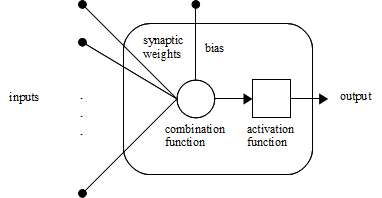
\includegraphics[width=0.85\textwidth]{neural_network/perceptron}
\caption{Perceptron neuron model.}\label{PerceptronFigure}
\end{center}
\end{figure}

Here we identify three
basic elements, which transform a vector of inputs into a single output \cite{Belanche2000}: 

\begin{description}
\item[(i)] A set of parameters consisting of a bias and a vector of synaptic weights.
\item[(ii)] A combination function.  
\item[(iii)] An activation function or transfer function.
\end{description}

\subsection*{Perceptron layer}

Most neural networks, even biological neural networks, exhibit a
layered structure \cite{Sima2003} \cite{Demuth2009}. In this work layers are the basis to
determine the architecture of a neural network.

A layer of perceptrons is composed by a set of perceptrons sharing the same inputs. 
The architecuture of a layer is characterized by the number of inputs and the number of perceptrons. 
Figure \ref{PerceptronLayerFigure} shows a general layer of perceptrons. 

\begin{figure}[h!]
\begin{center}
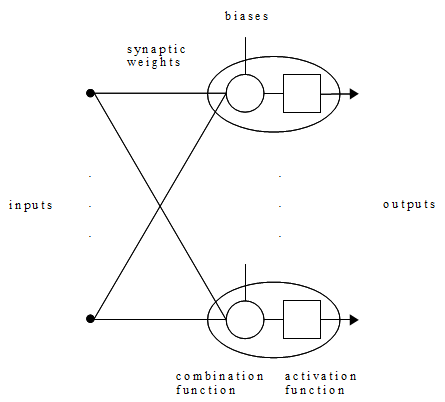
\includegraphics[width=0.9\textwidth]{neural_network/perceptron_layer}
\caption{Layer.}\label{PerceptronLayerFigure}
\end{center}
\end{figure}

Here we identify three basic elements, which transform a vector of inputs
into a vector of outputs: 

\begin{description}
\item[(i)] A set of layer parameters. 
\item[(ii)] A layer combination function.  
\item[(iii)] A layer activation function.
\end{description}


\subsection*{Multilayer perceptron}
\index{network architecture}
\index{feed-forward architecture}

\index{input variable name}
\index{input variable description}
\index{input variable units}

\index{output variable name}
\index{output variable description}
\index{output variable units}

\index{layer}
\index{input layer}
\index{hidden layer}
\index{output layer}
\index{composition diagram}

Layers of perceptrons can be composed to form a multilayer perceptron. Most neural networks, 
even biological ones, exhibit a layered structure. Here
layers and forward propagation are the basis to determine the architecture of a multilayer perceptron. This neural network represent an explicit function wich can be used for a variety of purposes. 

% Network architectture 

The architecture
of a multilayer perceptron refers to the number of neurons, their
arrangement and connectivity. Any
 architecture can be symbolized as a directed and labeled
graph, where nodes represent neurons and edges represent
connectivities among neurons. An edge label represents the
parameter of the neuron for which the flow goes in
\cite{Belanche2000}.

Thus, a neural network typically consists on a set of sensorial
nodes which constitute the input layer, one or more hidden layers of
neurons and a set of neurons which constitute the output layer.

There are two main categories of network architectures: acyclic or feed-forward networks 
and cyclic or recurrent networks \cite{Russell2009}. A feed-forward network represents 
a function of its current input; on the contrary, a recurrent neural network feeds outptus back into
its own inputs. 

As it was said above, the characteristic neuron model of the
multilayer perceptron is the perceptron. On the other hand, the
multilayer perceptron has a feed-forward network architecture.

Hence, neurons in a feed-forward neural network are
grouped into a sequence of layers of neurons, so that neurons in any layer are connected only to
neurons in the next layer. 

The input layer consists of external inputs and is not a layer of neurons; 
the hidden layers contain neurons; 
and the output layer is also composed of output neurons. 
Figure \ref{MultilayerPerceptronFigure} shows the network architecture of a multilayer perceptron. 

\begin{figure}[h!]
\begin{center}
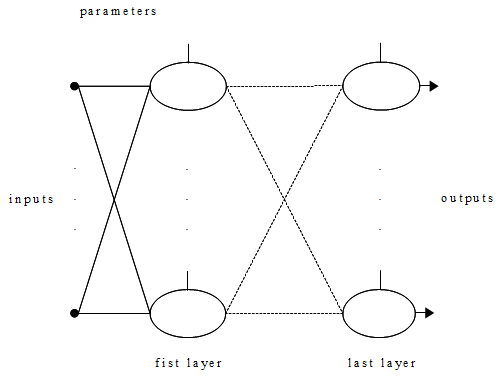
\includegraphics[width=1.1\textwidth]{neural_network/multilayer_perceptron}
\caption{Multilayer perceptron.}\label{MultilayerPerceptronFigure}
\end{center}
\end{figure}

A multilayer perceptron is characterized by:

\begin{description}
\item[(i)] A network architecture.
\item[(ii)] A set of parameters.
\item[(iii)] The layers activation functions.
\end{description}

Communication proceeds layer by layer
from the input layer via the hidden layers up to the output layer.
The states of the output neurons represent the result of the
computation \cite{Sima2003}.

In this way, in a feed-forward neural network, the output of each
neuron is a function of the inputs. Thus, given an input to such a
neural network, the activations of all neurons in the output layer
can be computed in a deterministic pass \cite{Bishop1995}.

\subsection*{Scaling layer}

In practice it is always convenient to scale the inputs in order to make all of them to be of order zero.
In this way, if all the neural parameters are of order zero, the
outputs will be also of order zero. On the other hand, scaled outputs are to be unscaled in order to produce the original units.

In the context of neural networks, the scaling function can be thought as an additional layer connected to the input layer of the multilayer perceptron. The number of scaling neurons is the number of inputs, and the connectivity of that layer is not total, but one-to-one. 

%Figure \ref{InputScalingLayerFigure} illustrates the input scaling layer. 

%\begin{figure}[h!]
%\begin{center}
%\includegraphics[width=0.5\textwidth]{neural_network/scaling_layer}
%\caption{Scaling layer.}\label{ScalingLayerFigure}
%\end{center}
%\end{figure}

The scaling layer contains some basic statistics on the inputs. They include the mean, standard deviation, minimum and maximum values.
Two scaling methods very used in practice are the minimum-maximum and the mean-standard deviation methods. 

\subsection*{Unscaling layer}

Also, scaled outputs from a multilayer perceptron are to be unscaled in order to produce the original units.
In the context of neural networks, the unscaling function can be interpreted as an unscaling layer connected to the outputs of the multilayer perceptron. 

%\begin{figure}[h!]
%\begin{center}
%\includegraphics[width=0.5\textwidth]{neural_network/unscaling_layer}
%\caption{Unscaling layer.}\label{UnscalingLayerFigure}
%\end{center}
%\end{figure}

The unscaling layer contains some basic statistics on the outputs. They include the mean, standard deviation, minimum and maximum values. 
Two unscaling methods very used in practice are the minimum-maximum and the mean-standard deviation methods. 

\subsection*{Bounding layer}
\index{output variables lower bounds}
\index{output variables upper bounds}

Lower and upper bounds are an essential issue for that problems in which some variables are restricted to fall in an interval. Those problems could be intractable if bounds are not applied. 

An easy way to treat lower and upper bounds is to post-process the outputs from the neural network with a bounding function.
That function can be also be interpreted as an additional layer connected to the outputs. 

%see Figure \ref{UnscalingLayerFigure}.

%\begin{figure}[h!]
%\begin{center}
%\includegraphics[width=0.5\textwidth]{neural_network/BoundingLayer}
%\caption{Bounding layer.}\label{BoundingLayerFigure}
%\end{center}
%\end{figure}

\subsection*{Probabilistic layer}

A probabilistic function takes the outputs to produce new outputs whose elements can be interpreted as probabilities. 
In this way, the probabilistic outputs will always fall in the range $[0,1]$, and the sum of all will always be $1$. This form of postprocessing is often used in patter recognition problems.

The probabilistic function can be interpreted as an additional layer connected to the output layer of the network architecture.

%\begin{figure}[h!]
%\begin{center}
%\includegraphics[width=0.5\textwidth]
%{neural_network/probabilistic_layer}
%\caption{Probabilistic layer.}\label{ProbabilisticLayerFigure}
%\end{center}
%\end{figure}

Note that the probabilistic layer has total connectivity, and that it does not contain any parameter. 
Two well-known probabilistic methods are the competitive and the softmax methods. 

\subsection*{Conditions layer}

If some outputs are specified for given inputs, then the problem is
said to include conditions. 

A conditions layer will be connected to the outputs of the multilayer perceptron. It will take both the input and the output values from that neural network to produce new outptus satisfying the conditions. 

Treatment of conditions is quite a difficult task. Here a particular and a homogeneous solutions are first derived. Then, both the inputs and the outputs from the multilayer perceptron are processed with the particular and homogeneous functions in order to hold the conditions. 

\subsection*{Independent parameters}

If some information not related to input-output relationships is
needed, then the problem is said to have independent parameters.
They are not a part of the neural network, but they are associated
to it. 

The independent parameters are grouped together in a vector. 

\subsection*{Neural network}

A neural network defines a function which is of the following form.

\begin{eqnarray}\nonumber
outputs = function(inputs). 
\end{eqnarray}


The most important element of an \texttt{OpenNN} neural network is the multilayer perceptron. 
That composition of layers of perceptrons is a very good function approximator. 

Many practical applications require, however, extensions to the multilayer perceptron. 
\texttt{OpenNN} presents a neural network with some of the most standard extensions. 
They include the scaling, uscaling, bounding, probabilistic or conditions layers.  

For instance, a function regression problem might require a multilayer perceptron with scaling and unscaling layers. 
On the other hand, an optimal control problem may need a multilayer perceptron with a conditions layer.

Finally, some problems might require the use of other adjustable parameters than those belonging to the multilayer perceptron. 
That kind of parameters are called independent parameters.

Some basic information related to the input and output variables of a neural network includes the name, description and units of that variables. That information will be used to avoid errors such as interchanging the role of the variables, misunderstanding the significance of a variable or using a wrong units system. 

